\documentclass{standalone}
\usepackage{tikz}
\usepackage{calc}
\usepackage{pgffor}
\usetikzlibrary{patterns}
\begin{document}
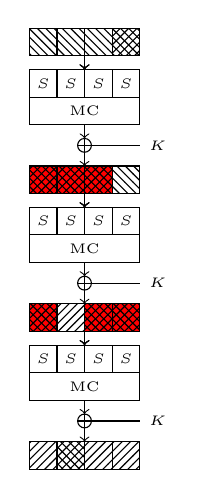
\begin{tikzpicture}[scale=0.35]
\begin{scope}[yshift = -5cm]
\fill[red](0,0) rectangle+(1,1);
\fill[red](1,0) rectangle+(1,1);
\fill[red](2,0) rectangle+(1,1);
\end{scope}
\begin{scope}[yshift = -10cm]
\fill[red](0,0) rectangle+(1,1);
\fill[red](2,0) rectangle+(1,1);
\fill[red](3,0) rectangle+(1,1);
\end{scope}
\begin{scope}[yshift = 0cm]
\draw[pattern = north west lines](0,0) rectangle+(1,1);
\draw[pattern = north west lines](1,0) rectangle+(1,1);
\draw[pattern = north west lines](2,0) rectangle+(1,1);
\draw[pattern = north east lines](3,0) rectangle+(1,1);
\draw[pattern = north west lines](3,0) rectangle+(1,1);
\end{scope}
\begin{scope}[yshift = -5cm]
\draw[pattern = north east lines](0,0) rectangle+(1,1);
\draw[pattern = north west lines](0,0) rectangle+(1,1);
\draw[pattern = north east lines](1,0) rectangle+(1,1);
\draw[pattern = north west lines](1,0) rectangle+(1,1);
\draw[pattern = north east lines](2,0) rectangle+(1,1);
\draw[pattern = north west lines](2,0) rectangle+(1,1);
\draw[pattern = north west lines](3,0) rectangle+(1,1);
\end{scope}
\begin{scope}[yshift = -10cm]
\draw[pattern = north east lines](0,0) rectangle+(1,1);
\draw[pattern = north west lines](0,0) rectangle+(1,1);
\draw[pattern = north east lines](1,0) rectangle+(1,1);
\draw[pattern = north east lines](2,0) rectangle+(1,1);
\draw[pattern = north west lines](2,0) rectangle+(1,1);
\draw[pattern = north east lines](3,0) rectangle+(1,1);
\draw[pattern = north west lines](3,0) rectangle+(1,1);
\end{scope}
\begin{scope}[yshift = -15cm]
\draw[pattern = north east lines](0,0) rectangle+(1,1);
\draw[pattern = north east lines](1,0) rectangle+(1,1);
\draw[pattern = north west lines](1,0) rectangle+(1,1);
\draw[pattern = north east lines](2,0) rectangle+(1,1);
\draw[pattern = north east lines](3,0) rectangle+(1,1);
\end{scope}
\foreach \z in {0,1,2}{
\begin{scope}[yshift = -\z* 5 cm]
\draw (0,0) grid +(4,1);
\foreach \y in {0,1,2,3}{\draw[->](2,0)--+(0,-0.5);
\draw(\y,-1.5) rectangle node{\tiny{$S$}} +(1,1);
}
\draw (0,-2.5) rectangle node{\tiny{MC}} +(4,1);
\draw[->] (2,-2.5)--+(0,-0.5);
\draw (1.75,-3.25)--+(0.5,0);
\draw (2,-3.25) circle (0.25);
\draw (4,-3.25) --(2.25,-3.25);
\node[right] at (4,-3.25) {\tiny{$K$}};
\draw[->](2,-3)--+(0,-1);
\end{scope}}
\end{tikzpicture}
\end{document}